\documentclass[12pt]{article}

\usepackage{amsmath}
\usepackage{amssymb}
\usepackage{hyperref}
\usepackage{xcolor}
\usepackage{tikz}

\begin{document}

\title{CS 7240 Project Report: CDCL SAT Solver Implementation}
\author{William Schultz}
\date{\today}

\maketitle

\newcommand{\green}[1]{\textcolor{green}{#1}}
\newcommand{\red}[1]{\textcolor{red}{#1}}

\section{Introduction}

Satisfiability (SAT) solvers have become powerful tools for solving hard, generic constraint satisfaction problems. Even though the SAT problem is known to be fundamentally hard (NP-complete), these tools are now effective at solving large, nontrivial real world problem instances and are applied widely in hardware and software verification, program analysis, electronic design automation, etc. The goal of this project was to implement a SAT solver based on relatively state of the art techniques, which are mostly based on \textit{conflict driven clause learning} (CDCL) \cite{09bieresathandbook, bierecdcl,96sakallah}, an extension of the foundational DPLL algorithm \cite{1960dpll}. The goal was to implement such a solver and compare its performance to other state of the art solvers, and to understand the underlying algorithms in more depth.

\section{Preliminaries}

The satisfiability problem is defined as follows. Given a boolean formula $f$ in conjunctive normal form (CNF), determine if there exists an assignment of values to the boolean variables of $f$ such that $f$ evaluates to true under this assignment. We want to return such a satisfying assignment, or determine that no such assignment exists. For example, the following CNF formula
\begin{align*}
    (x_1 \vee x_2) \wedge (\neg x_3 \vee \neg x_1)
\end{align*}
is satisfiable with assignment $\{x_1=1, x_2=0, x_3=0\}$. The standard convention is to view CNF formulas as sets of clauses, where a clause is simply a set of \textit{literals} i.e. a variable or its negation. Thus, the above formula can be represented as the set
\begin{align*}
    \{\{x_1,x_2\}, \{\neg x_3, \neg x_1\}\}
\end{align*}
Determining satisfiability of an arbitrary boolean formula in CNF is NP-complete \cite{71cook}.

\section{DPLL}

A basic approach to solving satisfiability is to view it as a search problem over possible assignments to variables. This is the basic idea behind the Davis–Putnam–Logemann–Loveland (DPLL) algorithm \cite{dpll1961}. The DPLL algorithm essentially performs a depth first, brute first search over the tree of possible assignments, performing basic formula simplifications as it extends partial assignments in its search. In particular, standard DPLL makes use of the \textit{unit propagation} rule. A clause of a CNF formula is a \textit{unit clause} if it contains exactly one literal. For a CNF that contains a unit clause $c$, we know that $c$ must be true in any possible satisfying assignment, so we must set the variable for the literal in $c$ accordingly. For example, consider the repeated application of unit propagation to the following formula:
\begin{align*}
    &\{\{b\}, \{\neg b, \neg c\}, \{c, \neg d\}\}\\
    &\{\{\green{b}\}, \{\red{\neg b}, \neg c\}, \{c, \neg d\}\}\\
    &\{\{\neg c\}, \{c, \neg d\}\} \\
    &\{\{\green{\neg c}\}, \{\red{c}, \neg d\}\}\\
    &\{\{\neg d\}\}\\
    &\{\{\green{\neg d}\}\}\\
    &\{\} \quad (\text{SAT})
\end{align*}
In this case, repeated application of unit propagation leads us to the empty formula, which, interpreted as an empty conjunction, is trivially satisfied. We also recover the satisfying assignment from this sequence of unit propagation applications i.e. $\{b=1,c=0,d=0\}$.

DPLL performs a depth first search in the tree of possible assignments, backtracking when it encounters a \textit{conflict}, which is defined as occurring when some clause has all of its literals set to \textit{false} in a current partial assignment. To illustrate the work done by a run of DPLL on a given formula, we can show its \textit{termination tree} \cite{09bieresathandbook}, which essentially shows the parts of the search tree that it explored during its run. For example, the termination tree for the following CNF formula (with each clause labeled):
\begin{align*}
    &c_1 \quad \{a,b\}\\
    &c_2 \quad \{b,c\}\\
    &c_3 \quad \{\neg a, \neg x, y\} \\
    &c_4 \quad \{\neg a, x, z\} \\
    &c_5 \quad \{\neg a, \neg y, z\} \\
    &c_6 \quad \{\neg a, x, \neg z\} \\
    &c_7 \quad \{\neg a, \neg y, \neg z\}
\end{align*}
is depicted in Figure \ref{fig:dpll-term-tree}. It shows the paths taken by DPLL, leading to conflicts at the red ``X" nodes, before it eventually finds a satisfying assignment where $\{a=0,b=1\}$.

\begin{figure}
    \begin{center}
    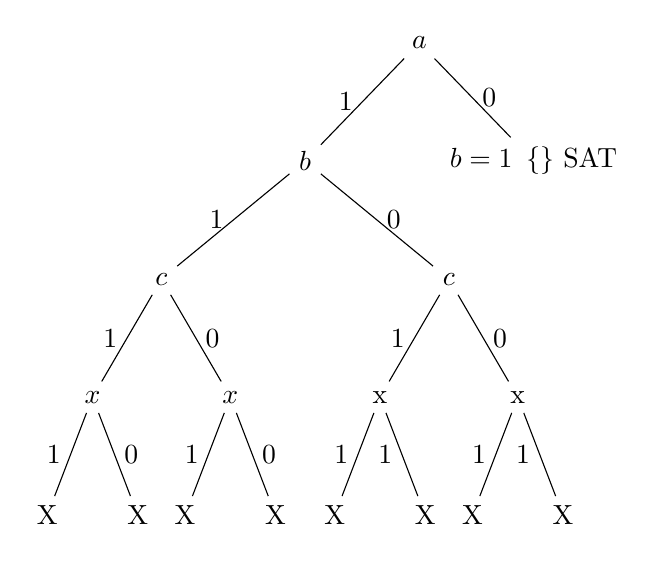
\begin{tikzpicture}
        \node {$a$} [sibling distance = 2.9cm]
        child [] {node {$b$} [sibling distance =3.65cm]
            % c=1
            child [] {node {$c$} [sibling distance = 1.75cm]
                child [] {node {$x$} [sibling distance = 1.15cm]
                    child [] {node {\red{X}} edge from parent [] node [left]{1}}
                    child [] {node {\red{X}} edge from parent [] node [right]{0}}
                edge from parent [] node [left]{1}} 
                child [] {node {$x$} [sibling distance = 1.15cm]
                    child [] {node {\red{X}} edge from parent [] node [left]{1}}
                    child [] {node {\red{X}} edge from parent [] node [right]{0}}
                edge from parent [] node [right]{0}}
            edge from parent [] node [left]{1}}
            % c=0
            child [] {node {$c$} [sibling distance =1.75cm]
                child [] {node {x} [sibling distance = 1.15cm]
                    child [] {node {\red{X}} edge from parent [] node [left]{1}}
                    child [] {node {\red{X}} edge from parent [] node [left]{1}}
                edge from parent [] node [left]{1}}
                child [] {node {x} [sibling distance = 1.15cm]
                    child [] {node {\red{X}} edge from parent [] node [left]{1}}
                    child [] {node {\red{X}} edge from parent [] node [left]{1}}  
                edge from parent [] node [right]{0}}
            % edge from parent [] node [left]{0}} 
            edge from parent [] node [right]{0}}
        edge from parent [] node [left]{1}}
        % a = 0.
        child [] {node {$b=1$\, $\{\}$ \green{SAT}} 
        edge from parent [] node [right]{0}};
    \end{tikzpicture}
    \end{center}
    \caption{DPLL termination tree.}
    \label{fig:dpll-term-tree}
\end{figure}

\section{Conflict Driven Clause Learning (CDCL)}

DPLL is a relatively naive algorithm, in the sense that it is fairly close to naive, brute force depth first search. An improvement to this framework that started being used in SAT solvers in the 1990s and 2000s is known as \textit{conflict driven clause learning} (CDCL) \cite{96sakallah,01zhangcdcl}. The technique is based around ideas of (1) \textit{learning from conflicts} and (2) \textit{non-chronological backtracking}. That is, when we encounter a conflict in a branch of the search tree, rather than simply backtracking naively to the most recent level and trying another path, we try to learn more about what variable settings caused this conflict, in an effort to avoid making similar mistakes again in other portions of the search tree. In addition, we backtrack \textit{non-chronologically}. That is, rather than backtracking to the previous level of the search tree, we try to jump back many levels, avoiding variables that were potentially irrelevant to the conflict we encountered.

\begin{figure}
    \begin{center}
    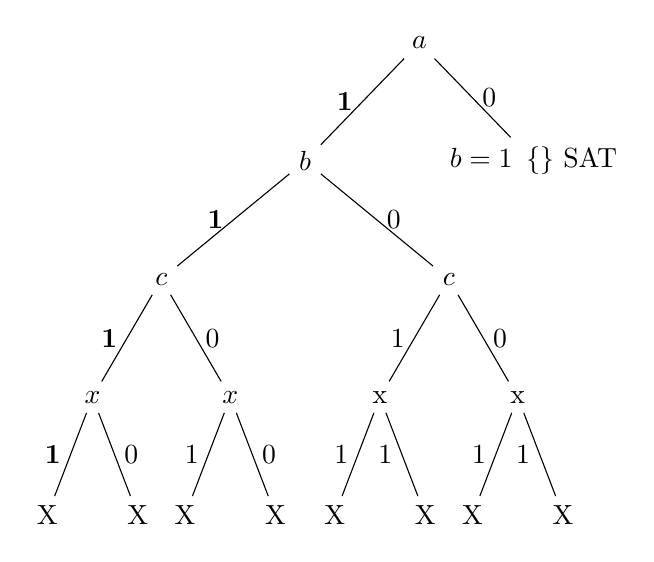
\begin{tikzpicture}
        \node {$a$} [sibling distance = 2.9cm]
        child [] {node {$b$} [sibling distance =3.65cm]
            % c=1
            child [] {node {$c$} [sibling distance = 1.75cm]
                child [] {node {$x$} [sibling distance = 1.15cm]
                    child [] {node {\red{X}} edge from parent [] node [left]{\textbf{1}}}
                    child [] {node {\red{X}} edge from parent [] node [right]{0}}
                edge from parent [] node [left]{\textbf{1}}} 
                child [] {node {$x$} [sibling distance = 1.15cm]
                    child [] {node {\red{X}} edge from parent [] node [left]{1}}
                    child [] {node {\red{X}} edge from parent [] node [right]{0}}
                edge from parent [] node [right]{0}}
            edge from parent [] node [left]{\textbf{1}}}
            % c=0
            child [] {node {$c$} [sibling distance =1.75cm]
                child [] {node {x} [sibling distance = 1.15cm]
                    child [] {node {\red{X}} edge from parent [] node [left]{1}}
                    child [] {node {\red{X}} edge from parent [] node [left]{1}}
                edge from parent [] node [left]{1}}
                child [] {node {x} [sibling distance = 1.15cm]
                    child [] {node {\red{X}} edge from parent [] node [left]{1}}
                    child [] {node {\red{X}} edge from parent [] node [left]{1}}  
                edge from parent [] node [right]{0}}
            % edge from parent [] node [left]{0}} 
            edge from parent [] node [right]{0}}
        edge from parent [] node [left]{\textbf{1}}}
        % a = 0.
        child [] {node {$b=1$\, $\{\}$ \green{SAT}} 
        edge from parent [] node [right]{0}};
    \end{tikzpicture}
    \end{center}
    \caption{Learning from conflicts in CDCL.}
    \label{fig:cdcl-term-tree}
\end{figure}

For example, if we look the termination tree from Figure \ref{fig:dpll-term-tree} we can consider what happens when the first, leftmost branch is explored by DPLL, as depicted in Figure \ref{fig:cdcl-term-tree}. We encounter a conflict in clause $c_7$ under the partial assignment of $\{a=1,b=1,c=1,x=1\}$, due to unit propagation being applied and triggering the additional assignments $\{y=1, z=1\}$. After encountering this conflict, naive DPLL would backtrack and try the next unexplored assignment to $x$. But, we can instead try to learn more information about why this conflict was encountered, in an effort to avoid making a similar mistake again in other regions of the search space. Specifically, we can see that, in fact, either $(a \wedge x)$ or $(a \wedge y)$ are both sufficient to lead to a conflict. So, we can implicitly encode this information as a new constraint in our original CNF formula. That is, we can simply add the negation $\neg (a \wedge x) = (\neg a \vee \neg x)$ as a new, \textit{learned clause}. Then, we can restart our search and treat the learned clause as if it were a normal clause of the original CNF formula. This is the basic intuition behind conflict driven clause learning. That is, when we encounter a conflict, we analyze it to derive a clause that we can learn, and then add this a new clause in our overall formula. In addition, we jump back in the search tree and restart, now with the newly learned clause as a part of our formula.

We can view the conflict analysis procedure more formally by looking at the \textit{implication graph} of variable assignments in a path of the search tree \cite{09bieresathandbook}. For example Figure \ref{fig:impl-graph} shows an implication graph corresponding to the leftmost search path depicted in Figure \ref{fig:cdcl-term-tree}. Nodes of this graph represent variable assignments, and edges represent dependencies between these assignments. That is, if a variable is assigned due to unit propagation, then it has incoming edges corresponding to the other variable assignments that caused it to become unit. Cuts in this graph then correspond to \textit{conflict sets}, which can be used to derive different learned clauses. In general, there may be many such cuts, and so many possible clauses to learn.

\begin{figure}
    \begin{center}
        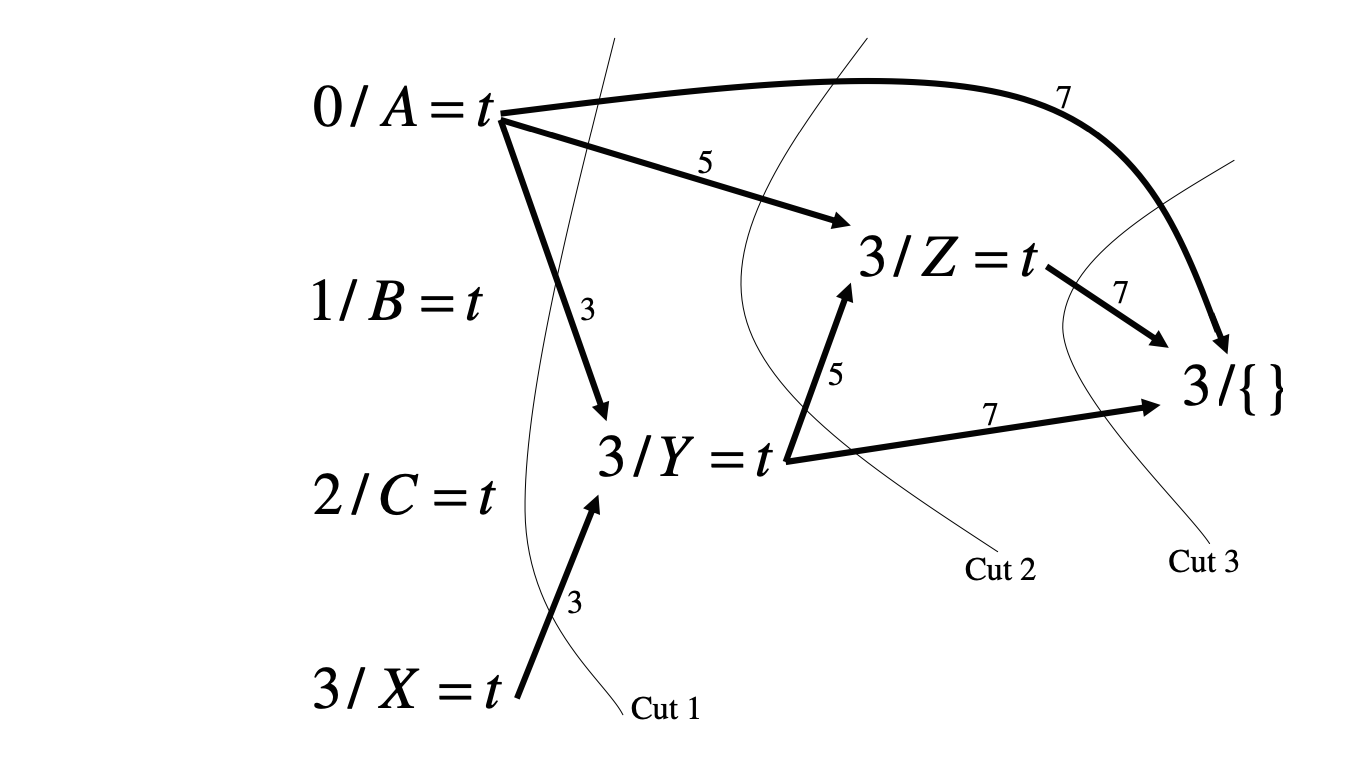
\includegraphics[scale=0.4]{figures/impl-graph.png}
    \end{center}
    \caption{Implication graph with 3 possible cuts.}
    \label{fig:impl-graph}
\end{figure}

\section{SAT Solver Implementation}

The large portion of work for this project consisted of implementing a basic, CDCL based SAT solver. The current version consists of approximately 1500 lines of C++, and the source code can be found at \url{https://github.com/will62794/mysat}, with the main solver logic found \href{https://github.com/will62794/mysat/blob/b721cb133098fd795219caa115cbae1cedf95ee2/sat.cpp}{here}. This code also includes an implementation of basic DPLL with unit propagation, in an effort to compare this approach with a basic version of CDCL.

As part of the implementation effort, the initial goal was to ensure correctness of the CDCL solver before trying to benchmark its performance. Correctness testing was performed by testing on randomly generated CNF formulas of varying sizes and with varying number of variables and clauses. In addition, the optimized, CDCL implementation was compared against a naive, brute force implementation to test conformance between the two implementations. This approach doesn't scale to large formulas, but works well for formulas with 10s of variables, since even a completely brute force solution can feasibly solve these instances.

\begin{figure}
    \begin{center}
        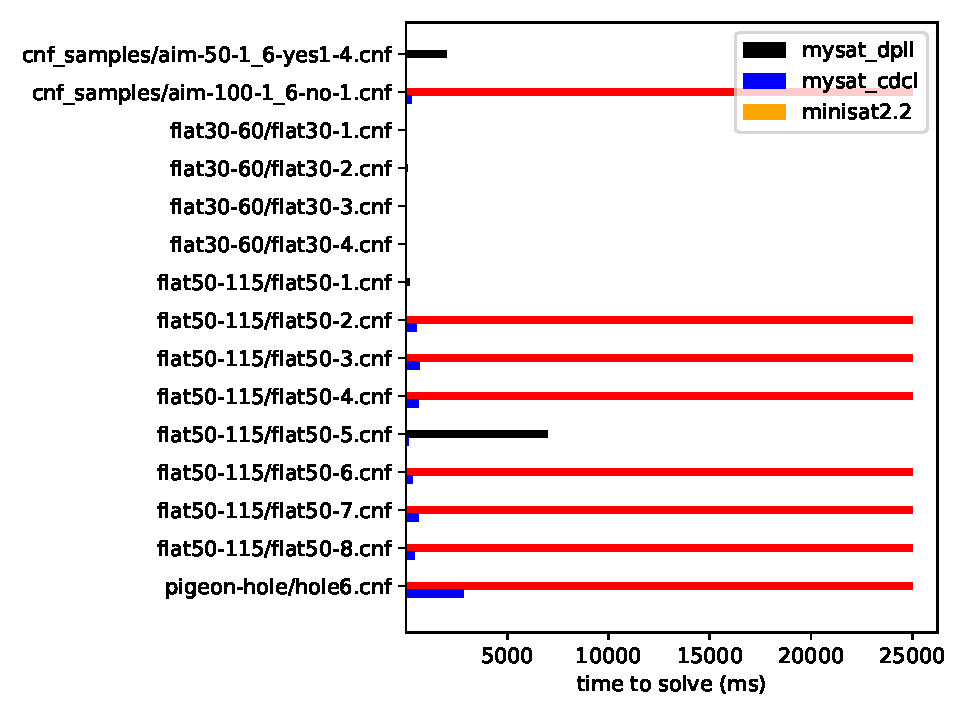
\includegraphics[scale=0.6]{../results/compare.pdf}
    \end{center}
    \caption{Preliminary comparison of our SAT solver implementation for both CDCL and DPLL variants against the MiniSAT 2.2 solver \cite{minisat}. }
    \label{fig:benchmarks}
\end{figure}

\section{Evaluation}

Our initial evaluation of solver performance consisted of testing a small set of graph coloring benchmarks using both our DPLL and CDCL implementation, and also comparing to MiniSAT version 2.2, which is not a state of the art solver by current standards but includes most of the core techniques used by modern state of the art solvers, and so is very performant relative to naive solver implementations. Our initial benchmarking results are shown in Figure \ref{fig:benchmarks}, where the x-axis displays time to solve a benchmark, or timeout within a fixed budget of 25 seconds, on a log scale. Red bars indiciate a timeout of the DPLL based implementation after 25 seconds. This small benchmark set includes a variety of graph coloring problem instances, with around 50-100 variables. In general, MiniSAT drastically outperforms our implementation, solving most benchmarks in under a few milliseconds, indicated by the fact that its bar is not even visible in most cases, even with a log scale. But, the evaluation does appear to provide evidence of the effectiveness of CDCL solving as compared to basic DPLL.

\section{Future Goals}

In future, the hope would be to explore new techniques for learning SAT heuristics, in the spirit of \textit{CrystalBall} \cite{2019sooscrystalball}, which applied a data driven approach to automatically learning heuristics for a solver. In particular heuristics for
\begin{enumerate}
    \item Variable ordering
    \item Learned clause deletion policies
    \item Random restarts
\end{enumerate}
would be the most interesting candidates to explore. Adding support for the output of DRAT resolution proofs \cite{2014dratproofs} for UNSAT cases in our SAT solver implementation would also be a desirable future goal.

\bibliographystyle{plain}
\bibliography{references}

\end{document}